\documentclass[12pt,letterpaper]{article}
\usepackage{graphicx}
\usepackage{xfrac}
\usepackage{mcode}
\usepackage{subcaption}
\captionsetup{compatibility=false}

\begin{document}

\title{HW3 Image Analysis by filter and Diffusion}
\author{Beichen Su}
\maketitle

\begin{abstract}
Using Filter and diffusion to analyze a set of pictures
This revised version includes bigger image to have a closer look.
\end{abstract}

\newpage
\section{Introduction and Overview}
GQ magazine is doing a feature article on VH1’s 3-time male model of the year Derek Zoolander (NOTE:If you haven’t watched this movie, then that is part of your homework too!). Much to every beautiful person’s dismay, the ridiculously good looking photos of Derek have created a crisis. First, ugly protesters against the fashion industry sweat shops in Eurasia have corrupted Derek’s touch-upped photos The only remaining photos are when Derek had a rash near his nose 
Help save Derek’s male modeling career!\\
task 1: Use filtering to try to clean up the corrupted images of Derek. Filter both the black and white image and the three levels of the RGB data of the color picture.\\
task 2: Use diffusion to locally try to remove Derek’s rash. You could potentially use both diffusion and filtering to get the best image quality. Again, you now have three diffusion equations to solve for the three levels of the color picture.\\
WE LOVE YOU DEREK!
\newline 




\section{Theoretical Background}
\subsection{Fourier analysis}
As with time–frequency analysis, the key idea is to decompose the image into its Fourier components.
This is easily done with a two-dimensional Fourier transform. Thus the image becomes
a collection of Fourier modes. Figure 1 shows a photo and its corresponding 2D Fourier transform.
The drawback of the Fourier transform is the fact that the Fourier transform of a sharp 
edged object results in a sinc-like function that decays in the Fourier modes like 1/k where k is
the wavenumber. This slow decay means that localization of the image in both the spatial and
wavenumber domain is limited. Regardless, the Fourier mode decomposition gives an alternative
representation of the image. Moreover, it is clear from the Fourier spectrum that a great number
of the Fourier mode components are zero or nearly so. Thus the concept of image compression
can easily be seen directly from the spectrum, i.e. by saving $ 20\% $ of the dominant modes only, the image can be nearly constructed. This then would compress the image five-fold. As one might also expect, filtering with the Fourier transform can also help process the image to some desired ends.
\begin{figure}[h]
	\caption{Image of a beautifully made cappuccino along with its Fourier transform (log of the absolute
		value of the spectrum) in two dimensions. The strong vertical and horizontal lines in the spectrum correspond
		to vertical and horizontal structures in the photo. Looking carefully at the spectrum will also reveal
		diagonal signatures associated with the diagonal edges in the photo.}
	\centering
	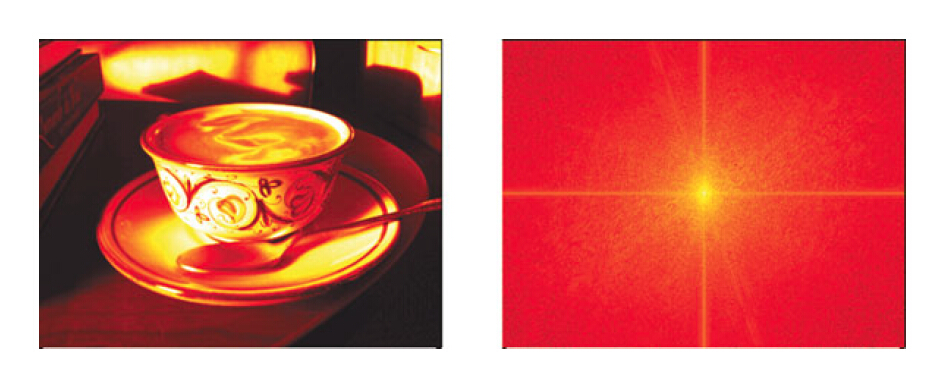
\includegraphics[width=0.5\textwidth]{book1}
\end{figure}


\subsection{Partial differential equations and diffusion}
For denoising applications, or applications in which the data is choppy or highly pixelated,
smoothing algorithms are of critical importance. In this case, one can take the original data as
the initial conditions of a diffusion process so that the image undergoes, in the simplest case, the evolution
\begin{equation}
\frac{\partial u}{\partial t} = D \bigtriangledown ^2 u
\end{equation}
where $\bigtriangledown ^2 = \partial_x ^2 \partial_y ^2$ This diffusion process provides smoothing to the original data file u. The
key is knowing when the smoothing process should be stopped so as not to remove too much
image content.

More theorem on text book p360.


\section{Algorithm Implementation and Development}
\subsection{Corrupted Image}
For dealing with black and white image in this part, we load the image into matlab, and it's a n by n matrix. By taking fourier transform of the image and taking log of the absolute value of it, we can find the highest frequency in fourier domain.
Then we build a gaussian filter on the highest frquency and with different width.
Have to mention that we have to notice if the image in  matchs the filter in fourier domain.
After applying the filter, we transform the image back and show the image.\\

For a color image, with RGB components, we do the same thing as we did in black and white, but 3 times for each layer. After doing all the filtering for 3 layers, we transform them back, combine them in a 3D data cube and do uint8 to view the image.

\subsection{Remove rash}
Starting at black and white image, by playing around the rash is located at $A(135:165,155:185)$, where A is the image we load. Then we build laplacian operation with spdiags command and use Kron function to do meshgrid in higher dimension. Then we build the diffusion constant, with entries 1 at the pixels of rash and 0 otherwise. Then do the reshape, run our ode solver and the rash is removed.\\

As for the color image, it's the same as we did in black and white version, but to do it for each layer and combine.


\section{Computational Results}

\subsection{part 1}
As shown in figure 2, fast fourier transform the image and log the absolute value, it's clear to see the most important data are at the center of the fourier domain. So that we build filters with different width on the center, to see how the width effects the outcome image, as shown in figure 3, at width equal to 0.001 we get the best image.\\
For the color image, the filter should still be built at the center of the fourier domain, as shown in figure 4. Applying filter and we get our clear image, as shown in figure 5, best image at width = 0.001.

\begin{figure}[h]
	\caption{BW: Original Image and frequency amplitude}
	\centering
	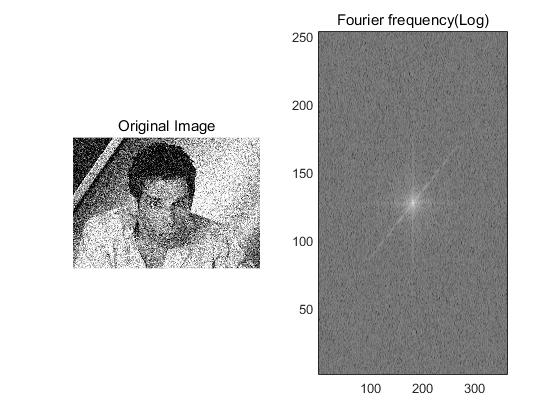
\includegraphics[width=1\textwidth]{Part1BW1}
\end{figure}

\begin{figure}[h]
	\caption{BW: Image after filtering with different width of gaussian filter}
	\centering
	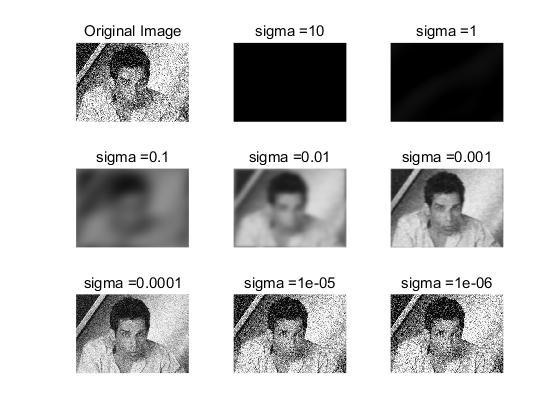
\includegraphics[width=1.4\textwidth]{Part1BW2}
\end{figure}

\begin{figure}[h]
	\caption{C: Original Amplitude}
	\centering
	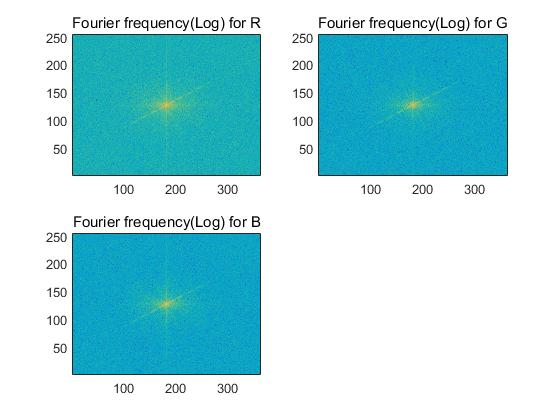
\includegraphics[width=1\textwidth]{Part1C1}
\end{figure}
\begin{figure}[h]
	\caption{C: Image after filtering with different width of gaussian filter}
	\centering
	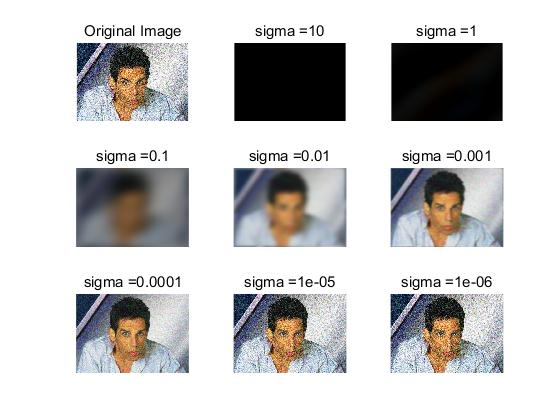
\includegraphics[width=1.4\textwidth]{Part1C2}
\end{figure}
\subsection{part 2}
Applying the diffusion by make the diffusion constant related to the x,y component, run the ode solver and we get our solution with clear face without rash as the diffusion time increases for both black and white and color image, as shown in figure 6 and 7.
	\begin{figure}[h]
		\caption{BW: Image after diffusion with diffusion constant = 0.001 at different diffusion time}
		\centering
		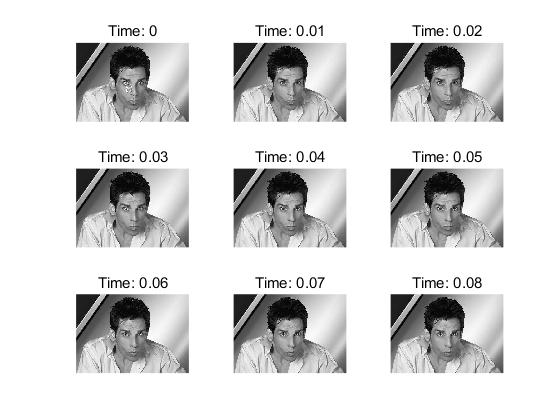
\includegraphics[width=1.4\textwidth]{Part2BW1}
	\end{figure}
\begin{figure}[h]
	\caption{C: Image after diffusion with diffusion constant = 0.001 at different diffusion time}
	\centering
	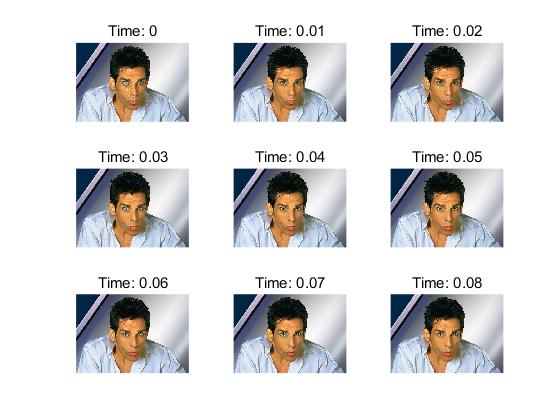
\includegraphics[width=1.4\textwidth]{Part2C1}
\end{figure}



\section{Conclusion}
By applying filter we can denoise a signal, and a image. It's important to understand the way that how information of an image stored and where to apply the filter.\\
As for 2D heat equation, the product of diffusion constant and the time t is the gaussian filter width. By making diffusion constant related to the x,y domain, we can clear a rash on the image rather than change the whole picture.





\appendix
\section{}
\subsection{linspace}
y = linspace(x1,x2,n) generates n points. The spacing between the points is (x2-x1)/(n-1).\\
In the code we have \\
$x2=linspace(-L,L,n+1);$\\
for FFT on a periodic boundary so the first point is the same as the last one. So we take n+1 mode and only pick the first n element.

\subsection{fft,fftshift,fftn}
fft,fft2,fftn transform the signal in 1D,2D and nD in to frequency domain with same dimension. When we do the tranformation, we must rescale the wavenumbers by $2*pi/L$ since the FFT assumes 2*pi periodic signals, where L is the spatial domain.

\subsection{meshgrid}
[X,Y,Z] = meshgrid(x,y,z) produces three-dimensional coordinate arrays. Make Matlab know your x, y ,z are perpendicular to each other.

\subsection{zeros, ones}
A = zeros(n,n,n) or ones(n,n,n) create a matrix with all zero and one entries with desired dimension

\subsection{reshape}
A = reshape(B,n,n) reshape a matrix with desired columns and rows

\subsection{max}
[m,I] = max(A);
A is a one dimensional matrix, m is the max number in the matrix and I is the index of m in A

\subsection{ind2sub}
The ind2sub command determines the equivalent subscript values corresponding to a single index into an array.

\subsection{kron}
$K = kron(A,B)$ returns the Kronecker tensor product of matrices A and B. If A is an m-by-n matrix and B is a p-by-q matrix, then kron(A,B) is an $m*p-by-n*q$ matrix formed by taking all possible products between the elements of A and the matrix B.

\subsection{uint8}
intArray = uint8(array) converts the elements of an array into unsigned 8-bit (1-byte) integers of class uint8.

\subsection{spdiags}
The spdiags function generalizes the function diag. Four different operations, distinguished by the number of input arguments, are possible.

\section{}


\begin{lstlisting}
% Here's the function of rhs
function rhs = image_rhs(t,A,dummy,L,D)
rhs = (L*A).*D;
end




clear all; close all; clc
% %% Part one - Black and white
% % Black and white image with filter
% figure(1)
% An = imread('derek2','jpeg');
% subplot(1,2,1)
% 
% imshow(An)
% title('Original Image')
% [nx,ny] = size(An);
% 
% % FFT the image
% Ant = fft2(An);
% figure(1)
% subplot(1,2,2)
% pcolor(log(abs(fftshift(Ant)) + 1)), shading interp
% title('Fourier frequency(Log)')
% 
% % Turns out the highest frequency at the center of the fourier domain
% % Where to apply a gaussian filter
% xcent = nx/2;
% ycent = ny/2;
% 
% % Create a gaussian filter with certain width
% kx = 1 : nx; ky = 1 : ny;
% [Kx,Ky] = meshgrid(kx,ky);
% figure(2)
% subplot(3,3,1)
% imshow(An)
% title('Original Image')
% sigma = 100;
% for j = 2 :9
% sigma = sigma/10;
% F = exp(-sigma*(Kx - xcent).^2 - sigma*(Ky - ycent).^2);
% % Shift the filter to fit the fft domain
% Fs = fftshift(F);
% Atf = Ant.* Fs';
% 
% % Transform back
% Af = ifft2(Atf);
% A = uint8(Af);
% subplot(3,3,j)
% imshow(A);
% title(['sigma =' num2str(sigma)]);
% end

% %% Part two - Color image
% AA = imread('derek1','jpeg');
% An = double(AA);
% % take out each layer of the data cube
% Rn = An(:,:,1);
% Gn = An(:,:,2);
% Bn = An(:,:,3);
% [nx,ny] = size(Bn);
% % Do fft to find where to apply filter
% % for R:
% figure(1)
% Rnt = fft2(Rn);
% subplot(2,2,1)
% pcolor(log(abs(fftshift(Rnt)) + 1)), shading interp
% title('Fourier frequency(Log) for R')
% 
% Gnt = fft2(Gn);
% subplot(2,2,2)
% pcolor(log(abs(fftshift(Gnt)) + 1)), shading interp
% title('Fourier frequency(Log) for G')
% 
% Bnt = fft2(Bn);
% subplot(2,2,3)
% pcolor(log(abs(fftshift(Bnt)) + 1)), shading interp
% title('Fourier frequency(Log) for B')
% 
% % Turns out still at the center of fourier domain
% % Apply filter 
% xcent = nx/2;
% ycent = ny/2;
% kx = 1 : nx; 
% ky = 1 : ny;
% [Kx,Ky] = meshgrid(kx,ky);
% 
% % Apply different filter width 
% sigma = [100 10 1 0.1 0.01 0.001 0.0001 0.00001 0.000001]
% figure(2)
% subplot(3,3,1)
% imshow(AA)
% title('Original Image')
% for ii = 2:length(sigma)
% F = exp(-sigma(ii)*(Kx - xcent).^2 - sigma(ii)*(Ky - ycent).^2); 
% % convert the filter in to fourier domain
% Fs = fftshift(F);
% A = zeros(nx,ny,3);
% % Filter each layer for RGB
% for j = 1:3
%     Ant = fft2(An(:,:,j));
%     Ants = Ant;
%     Antsf = Ants.*Fs';
%     A(:,:,j) = ifft2(Antsf);
% end
% subplot(3,3,ii)
% imshow(uint8(A));
% title(['sigma =' num2str(sigma(ii))]);
% end

% %% Part two - Black and white
% clear all, close all, clc
% A = imread('derek4', 'jpeg');
% 
% A = double(A);
% [nx,ny] = size(A);
% x = linspace(0,1,nx); dx = x(2) - x(1);
% y = linspace(0,1,ny); dy = y(2) - y(1);
% 
% onex = ones(nx,1); oney = ones(ny,1);
% % track only non-zero entries
% % second derivative in x direction
% Dx = (spdiags([onex -2*onex onex],[-1 0 1], nx, nx)/dx^2);
% Ix = eye(nx);
% % in y direction
% Dy = (spdiags([oney -2*oney oney],[-1 0 1], ny, ny)/dy^2);
% Iy = eye(ny);
% 
% % make the meshgrid for derivative
% L=kron(Iy,Dx)+kron(Dy,Ix);
% % make D with xy domain
% % By playing around find that the rash is on 
% % A(135:165,155:185)
% D = zeros(size(A));
% for j = 135:165
%     for jj = 155:185
%         D(j,jj) = 1;
%     end
% end
% 
% An0 = reshape(A,nx*ny,1);
% tspan = [0 0.01 0.02 0.03 0.04 0.05 0.06 0.07 0.08];
% Dc = 0.001;
% D = Dc*D;
% Ds = reshape(D, nx*ny, 1);
% [t,A_sol] = ode45('image_rhs',tspan, An0,[],L,Ds);
% 
% % pull the vector out in to matrix
% figure(1)
% for j = 1:9
%     subplot(3,3,j)
%     Aclean = uint8(reshape(A_sol(j,:),nx,ny));
%     imshow(Aclean);
%     title(['Time: ', num2str(tspan(j))]);
% end

%% Part two - diffusion with RGB
clear all;close all; clc
A = imread('derek3', 'jpeg');
A = double(A);
[nx,ny,nz] = size(A);
x = linspace(0,1,nx); dx = x(2) - x(1);
y = linspace(0,1,ny); dy = y(2) - y(1);

onex = ones(nx,1); oney = ones(ny,1);
% track only non-zero entries
% second derivative in x direction
Dx = (spdiags([onex -2*onex onex],[-1 0 1], nx, nx)/dx^2);
Ix = eye(nx);
% in y direction
Dy = (spdiags([oney -2*oney oney],[-1 0 1], ny, ny)/dy^2);
Iy = eye(ny);

% make the meshgrid for derivative
L=kron(Iy,Dx)+kron(Dy,Ix);

% make D with xy domain
% By playing around find that the rash is on 
% A(135:165,155:185)
D = zeros(nx,ny);
for j = 135:165
for jj = 155:185
D(j,jj) = 1;
end
end
tspan = [0 0.01 0.02 0.03 0.04 0.05 0.06 0.07 0.08];
Dc = 0.001;
D = Dc*D;
Ds = reshape(D, nx*ny, 1);
R = A(:,:,1);
G = A(:,:,2);
B = A(:,:,3);
Rn0 = reshape(R,nx*ny,1);
Gn0 = reshape(G,nx*ny,1);
Bn0 = reshape(B,nx*ny,1);
[t,R_sol] = ode45('image_rhs',tspan, Rn0,[],L,Ds);
[t,G_sol] = ode45('image_rhs',tspan, Gn0,[],L,Ds);
[t,B_sol] = ode45('image_rhs',tspan, Bn0,[],L,Ds);

figure(1)
A_sol = zeros(size(A));
for j = 1:9
A_sol = zeros(size(A));
subplot(3,3,j)
Rc = reshape(R_sol(j,:),nx,ny);
Gc = reshape(G_sol(j,:),nx,ny);
Bc = reshape(B_sol(j,:),nx,ny);
A_sol(:,:,1) = Rc;
A_sol(:,:,2) = Gc;
A_sol(:,:,3) = Bc;

imshow(uint8(A_sol));
title(['Time: ', num2str(tspan(j))]);
end

\end{lstlisting}
\end{document}